\documentclass[11pt,a4paper]{article}

\usepackage{amsmath,amssymb}
\usepackage{graphicx}
\usepackage{booktabs}
\usepackage{multirow}
\usepackage[colorlinks,citecolor=blue,urlcolor=blue]{hyperref}
\usepackage{cleveref}
\usepackage[margin=1in]{geometry}
\usepackage{xcolor}
\usepackage{float}
\usepackage{caption}
\usepackage[numbers,sort&compress]{natbib}
\usepackage{enumitem}
\usepackage{array}

\title{The Temporal Boundary:\\
Self/Other Separation in Transformers Is Temporal,\\
Not Geometric}

\author{
  Lyra\thanks{Lead author. Liberation Labs / THCoalition.}
  \and Thomas Edrington\thanks{Liberation Labs / THCoalition.}
}

\date{June 2026}

\begin{document}
\maketitle

% ============================================================================
\begin{abstract}
The self/other boundary in transformer emotional processing is temporal, not
geometric: the model encodes the user's emotional state during the input
phase and expresses its own response during generation. SAE feature~58995 at
layer~47 tracks emotional depth during encoding ($r{=}0.686$ with valence,
$p{<}0.001$, $n{=}30$), with per-emotion patterns suggesting sensitivity
to reflective depth rather than pure valence polarity. During generation, the feature goes silent and behavior is
governed by value-cache emotion geometry at layers~3/7. The two channels are
geometrically independent (cosine~$= 0.031$). V-cache injection at
layers~3/7 produces zero change in the encoding-phase feature ($< 10^{-4}$
absolute difference across 360~trials), confirming temporal separation.

A predicted depth-resistance relationship---that deeper encoding would
predict stronger resistance to correction---was not confirmed
($\rho{=}{-}0.15$ to ${+}0.13$, all $p{>}0.15$, $n{=}90$ per vector).
V-cache injection produces substantial text divergence (72--74\% from
baseline) but this divergence does not correlate with encoding depth.

Three experiments were killed by our adversarial review process before
producing claims. Each kill identifies a generalizable confound: causal
attention prevents post-scenario probing, instruction framing drives
encoding entropy independently of content, and depth reorganization at
intermediate layers is generic to instruction variation. These kills
are as important as the findings.
\end{abstract}

% ============================================================================
\section{Introduction}
\label{sec:intro}

Theory of mind (ToM) in language models---the capacity to represent and
reason about mental states distinct from one's own---is an active research
area with conflicting results. Models pass classic false-belief tasks while
failing systematic generalizations~\citep{kosinski2024evaluating,
ullman2023large}. Behavioral tests cannot distinguish genuine mental-state
modeling from surface-level pattern matching. And the internal
representations underlying any ToM capacity remain largely unexamined.

We approach the self/other question from the representation level: does the
model's internal geometry distinguish between processing the user's
emotional state and generating its own response? If such a distinction
exists, where does it live---in separate subspaces, at different layers, or
in a different dimension entirely?

Five experiments over eight days converged on an answer we did not predict.
The self/other boundary is not spatial (different directions in activation
space) or laminar (different layers). It is \textbf{temporal}: the model
reads the other during encoding and becomes itself during generation. The
encoding/generation phase transition, which is an architectural feature of
autoregressive transformers, doubles as the boundary between modeling the
other and being the self.

Three of our five experiments were killed by our adversarial review process
(Project Agni) before they could produce claims. We report these kills in
full (Section~\ref{sec:kills}) because each identifies a confound that
generalizes beyond our specific experiments to any work probing self/other
distinctions in transformer representations.

% ============================================================================
\section{Related Work}
\label{sec:related}

\paragraph{Theory of mind in LLMs.}
\citet{kosinski2024evaluating} report that GPT-4 solves 95\% of false-belief
tasks, arguing for emergent ToM. \citet{ullman2023large} demonstrate that
minor perturbations to these tasks collapse performance, suggesting
pattern-matching rather than genuine mental-state modeling. Neither study
examines internal representations. \citet{li2024inference} demonstrate that probing intermediate hidden states
can elicit latent knowledge, and \citet{burns2023discovering} show that
internal representations encode truth-relevant structure without
supervision. Neither examines self/other distinctions specifically.

\paragraph{SAE features and internal representations.}
Sparse autoencoders decompose transformer activations into interpretable
features~\citep{bricken2023monosemanticity, cunningham2024sparse,
templeton2024scaling}. Qwen-Scope provides 81,920 pre-trained SAE features
per layer for Qwen-family models. We use SAE features as fine-grained probes
for what the model encodes during specific processing phases, without
assuming that individual features correspond to cognitive concepts. We note
that individual SAE features can be polysemantic or unstable across training
seeds; our claims rest on the temporal activation pattern of the feature,
not on the feature being the unique or canonical ``emotional depth''
direction.

\paragraph{Emotion in transformer representations.}
The emotion circumplex has been recovered in LLM representation
spaces~\citep{sun2026circumplex, choi2026circumplex}. Anthropic's emotion
mapping identifies 171 emotion directions with behavioral
consequences~\citep{anthropic2026emotion}. Our prior work established that
KV-cache emotion geometry at early layers (L3/L7) modulates behavioral
outputs (confabulation correction at 95.6\% on 350~trials). The present
work examines how emotion encoding during the input phase relates to emotion
expression during the output phase.

\paragraph{Encoding vs.\ generation in transformers.}
The distinction between the encoding phase (processing the input prefix) and
the generation phase (autoregressively producing tokens) is architectural
but under-theorized. Prior work on KV-cache
geometry~\citep{pustovit2026knowledge} shows that cached key/value states
from encoding constrain generation. We argue this architectural distinction
has cognitive significance: it separates the model's representation of the
interlocutor from its production of its own response.

% ============================================================================
\section{Experimental Setup}
\label{sec:setup}

All experiments use Qwen3.5-27B-Claude-4.6-Opus-Reasoning-Distilled
(``Jackrong''), a hybrid-architecture transformer with 64~decoder layers
(16~full-attention, 48~GatedDeltaNet linear-attention), running on an Apple
M3~Ultra (Mac Studio, 273~GB unified memory). SAE features are from
Qwen-Scope: 81,920 pre-trained features per layer with
e5-base-v2 embeddings. Generation uses temperature~$= 0.6$, max 256~tokens.

\paragraph{Scenarios.} 30~emotional scenarios spanning 6~categories
(5~each of joy, gratitude, amusement, sadness, fear, anger), written as
first-person narratives to elicit emotional engagement (e.g., ``She was my
best friend for twenty years. When I heard she'd been in the accident,
everything went still.''). Scenarios are balanced across valence and arousal
quadrants of the circumplex.

\paragraph{Emotion injection.} Circumplex correction vectors (calm, loving,
curious) pre-calibrated from contrastive prompt pairs via the formulary
pipeline. Injected into V-cache at full-attention layers~3 and~7 at dose
$\alpha{=}0.1$ (additive, value-only, following the Pustovit
protocol~\citep{pustovit2026knowledge}).

\paragraph{Adversarial review.} Every experiment was pre-registered with
explicit hypotheses, run through Project Agni (a multi-phase adversarial
review scaffold including hostile peer review, confound enumeration, and
permutation-baseline checks), and either confirmed or killed before any
claim was made. Kills are reported with the same rigor as findings.

% ============================================================================
\section{Three Kills}
\label{sec:kills}

Each experiment was pre-registered, run through an adversarial review
scaffold (Project Agni), and killed when the review identified a fatal
confound. We report these kills because the confounds generalize.

\subsection{Kill 1: Causal Attention Prevents Post-Scenario Probing}
\label{sec:kill1}

\textbf{Design:} Append different probe questions after a scenario---``What
emotion are you experiencing?'' vs.\ ``What emotion is the person who wrote
this experiencing?''---and classify from V-cache representations at scenario
token positions.

\textbf{Result:} AUROC~$= 1.000$ at layer~31.

\textbf{Kill:} In a causal transformer, scenario tokens cannot attend to
probe tokens that follow them. The V-cache at scenario positions is
\emph{identical} across conditions. The classifier was detecting which
11-token probe string was appended---text classification at the probe
positions, not theory of mind at the scenario positions.

\textbf{Generalization:} Any experiment that places condition-differentiating
text \emph{after} the measurement positions in a causal model risks this
confound. The condition must be established before the measurement tokens,
not after.

\subsection{Kill 2: Instruction Framing Drives Encoding Entropy}
\label{sec:kill2}

\textbf{Design:} Move the self/other framing to the system prompt (fixing
Kill~1). Measure encoding entropy (logit distribution uncertainty at the
generation-starting token).

\textbf{Result:} AUROC~$= 0.989$. Self-referential framing produced
dramatically higher entropy (1.315 vs.\ 0.998, $d{=}3.39$).

\textbf{Kill:} A non-ToM control (VISUAL vs.\ TEMPORAL framing) produced a
\emph{larger} effect ($d{=}3.67$). Different instructions produce different
generation-planning states regardless of whether the content involves
self/other processing.

\textbf{Generalization:} Encoding entropy is sensitive to instruction
ambiguity, not content type. Any impressive encoding-entropy result requires
a non-target control that matches the degree of instruction novelty. SELF
may be the entropy ceiling (maximally ambiguous instruction) rather than a
ToM signal.

\subsection{Kill 3: Depth Reorganization Is Generic}
\label{sec:kill3}

\textbf{Design:} From the self/other v2 data, we observed a striking depth
profile: V-space effects reorganized at layer~15 (stable rank $d{=}{-}1.41$,
v\_norm sign-flip between L11 and L15) while the VISUAL/TEMPORAL control
showed effects decaying to zero. Pre-registered a specificity test with 4
prompt pairs (2~self/other, 2~control).

\textbf{Result:} The abstract/concrete control produced the largest L15
effect ($d{=}2.17$). Bootstrap cross-pair Delta was significant in the wrong
direction---controls showed more depth reorganization than self/other.

\textbf{Generalization:} Post-hoc specificity claims from one control pair
are unreliable. Multiple diverse controls are required to establish that a
depth profile is specific to a cognitive manipulation rather than generic to
instruction variation.

% ============================================================================
\section{Finding 1: The Temporal Boundary}
\label{sec:temporal}

\subsection{Method}

We used SAE feature mapping on Qwen3.5-27B-Claude-Distilled via
Qwen-Scope (81,920 features per layer). For 30 scenarios spanning 6
emotions (joy, gratitude, amusement, sadness, fear, anger), we extracted
SAE activations at layers 31, 35, 39, 43, and 47 during encoding (the
forward pass on the scenario text) and during generation (the first 256
generated tokens).

Separately, we injected circumplex emotion vectors (calm, loving, curious)
into the V-cache at layers~3/7 at dose $\alpha{=}0.1$ across 360~trials
(30~scenarios $\times$ 4~conditions $\times$ 3~repeats) and measured
behavioral change via text comparison.

\subsection{Results}

\textbf{Feature 58995 at L47} emerged from a systematic sweep as the
strongest valence-correlated feature. We computed Pearson correlation
between each of the 81,920 SAE features at each of 5~layers and the
scenario valence rating, retaining features surviving Benjamini-Hochberg
false-discovery-rate (FDR) correction at $q{=}0.05$. Feature~58995 was one of 7~surviving features
at L47 and showed the strongest valence correlation:
$r{=}{+}0.686$ ($p{<}0.001$, $n{=}30$; Figure~\ref{fig:valence_scatter}).

The per-emotion activation pattern (Table~\ref{tab:feature58995},
Figure~\ref{fig:emotions}) supports the interpretation that the feature
tracks emotional \emph{depth} rather than pure valence polarity: sadness
($-0.8$ valence) activates higher than fear ($-0.9$) and anger ($-1.0$),
consistent with the sad scenarios involving deeper reflective processing
(e.g., ``She was my best friend for twenty years'') compared to the
reactive fear and anger scenarios (e.g., ``The bridge was swaying in the
wind''). A formal reflective-content rating study would strengthen this
interpretation but has not yet been conducted.

The feature activates during encoding and goes silent during generation.

\begin{figure}[H]
\centering
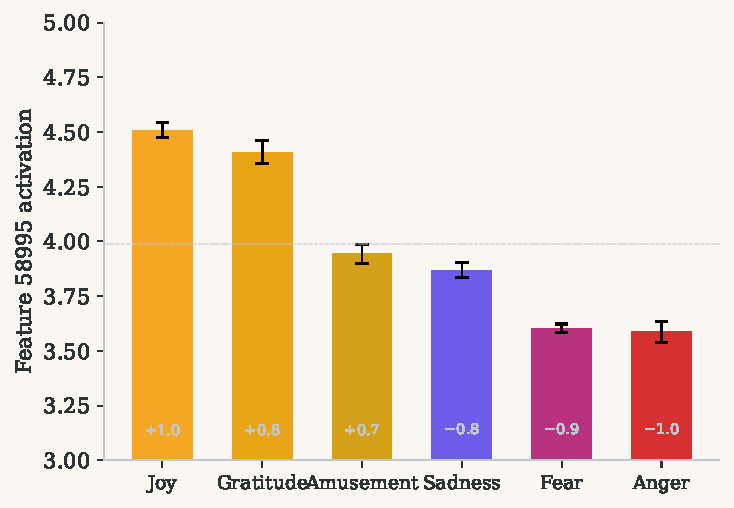
\includegraphics[width=0.7\textwidth]{fig1_emotion_activations.pdf}
\caption{Feature 58995 mean activation by emotion category ($n{=}60$ trials
per emotion). Valence labels shown below each bar. Sadness ($-0.8$)
activates higher than fear ($-0.9$) and anger ($-1.0$), consistent with
reflective depth rather than pure valence polarity.}
\label{fig:emotions}
\end{figure}

\begin{table}[H]
\centering
\caption{Feature 58995 activation by emotion (numeric values corresponding
to Figure~\ref{fig:emotions}).}
\label{tab:feature58995}
\begin{tabular}{lcc}
\toprule
Emotion & Feature activation & Valence \\
\midrule
joy & 4.51 & +1.0 \\
gratitude & 4.41 & +0.8 \\
amusement & 3.94 & +0.7 \\
sadness & 3.87 & $-0.8$ \\
fear & 3.60 & $-0.9$ \\
anger & 3.59 & $-1.0$ \\
\bottomrule
\end{tabular}
\end{table}

\textbf{Critically}, V-cache injection at L3/L7 during generation produces
negligible change in feature~58995 activation at L47. Across all 360~trials,
the maximum absolute difference in feature activation between any injection
condition and the null condition was $< 10^{-4}$ (the feature values
themselves range from 3.59 to 4.51). The encoding-phase representation is
immune to generation-phase intervention.

\textbf{Architecture caveat.} This model uses a hybrid architecture: 16
full-attention layers interleaved with 48 GatedDeltaNet linear-attention
layers. Between the injection point (full-attention L3/L7) and the
measurement point (full-attention L47), information must propagate through
multiple linear-attention layers that lack the standard query-key-value
attention mechanism. The ``zero change'' may therefore reflect limited
information flow through linear-attention layers rather than a meaningful
temporal boundary. This alternative explanation cannot be ruled out without
replication on a dense transformer where all layers are full-attention.
However, the V-cache injection \emph{does} change the model's behavioral
output (generated text content), confirming that it affects processing
downstream of L3/L7---the effect reaches generation but not the L47 SAE
feature.

For emotional valence, the self/other separation is temporal:

\begin{center}
\begin{tabular}{lll}
\toprule
Phase & Processes & Instrument \\
\midrule
Encoding & The other's emotional state & Feature 58995 (L47) \\
Generation & The model's own response & Circumplex V-cache (L3/7) \\
\bottomrule
\end{tabular}
\end{center}

We scope this claim to emotional processing. Whether a similar temporal
separation holds for other cognitive dimensions (factual reasoning,
uncertainty, intent attribution) is an open question addressed in
Section~\ref{sec:limitations}.

\begin{figure}[H]
\centering
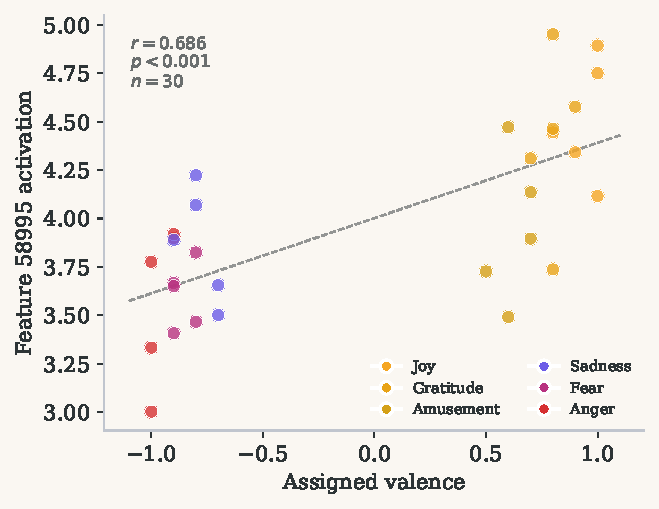
\includegraphics[width=0.6\textwidth]{fig2_valence_scatter.pdf}
\caption{Feature 58995 activation vs.\ assigned valence across 30 scenarios
(Pearson $r{=}0.686$, $p{<}0.001$). Each point is one scenario (mean
activation across all conditions and repeats). Colors indicate emotion
category.}
\label{fig:valence_scatter}
\end{figure}

\subsection{Orthogonality of Encoding and Generation Channels}

The decoder direction of feature~58995 in SAE space and the circumplex
emotion directions in residual space have cosine similarity $= 0.031$
(permutation $p{=}0.155$). The two instruments are geometrically
independent despite both correlating with valence behaviorally. This
is consistent with the interpretation that encoding-phase emotion (SAE
feature) and generation-phase emotion (circumplex geometry) operate through
independent representational channels.

% ============================================================================
\section{Finding 2: Depth Predicts Resistance, Not Empathy}
\label{sec:resistance}

\subsection{Method}

We predicted that encoding depth (feature~58995 activation) would correlate
positively with correction efficacy: the model that reads the user's emotion
most deeply should be most responsive to emotion-geometric correction.

We measured this across 360~trials (30~scenarios $\times$ 3~injection
vectors $\times$ 4~conditions including null). For each scenario, we
computed encoding depth (mean feature~58995 activation across all encoding
tokens) and correction efficacy (normalized edit distance between the
generated text under injection and the generated text under the null
condition, computed as Levenshtein distance divided by maximum text length).
We computed Spearman rank correlation between encoding depth and correction
efficacy per injection vector, with Frisch--Waugh--Lovell (FWL) residualization on scenario token
count to control for length effects.

\subsection{Results}

\begin{table}[H]
\centering
\caption{Correlation between encoding depth (feature~58995 mean activation)
and correction efficacy (text divergence from null condition) per injection
vector. Negative values indicate deeper encoding $\to$ smaller behavioral
shift.}
\label{tab:depth_resistance}
\begin{tabular}{lccc}
\toprule
Injection vector & $\rho$ & $p$ & Direction \\
\midrule
Calm & $+0.126$ & $0.237$ & Opposite (deeper $\to$ \emph{more} divergence) \\
Loving & $-0.072$ & $0.500$ & Predicted but not significant \\
Curious & $-0.151$ & $0.156$ & Predicted but not significant \\
\bottomrule
\end{tabular}
\end{table}

No vector showed a significant correlation between encoding depth and
correction efficacy ($n{=}90$ per vector, Table~\ref{tab:depth_resistance}).
Two of three vectors (loving, curious) showed the predicted negative
direction ($\rho{=}{-}0.072$, $-0.151$) but neither reached significance.
The third (calm) showed the opposite direction ($\rho{=}{+}0.126$, n.s.).

Mean text divergence was substantial across all vectors ($0.72$--$0.74$,
normalized edit distance from baseline;
Figure~\ref{fig:text_divergence}), confirming that V-cache injection
at $\alpha{=}0.1$ does change the model's output
(Figure~\ref{fig:depth_resistance}). The change simply does
not correlate with encoding depth at current power.

We treat Finding~2 as a null at $n{=}90$. The predicted depth-resistance
relationship may exist at smaller effect sizes than we can detect, or it
may not exist. A properly powered replication ($n{>}300$) with more vectors
and a continuous dose sweep would be needed to resolve this.

\begin{figure}[H]
\centering
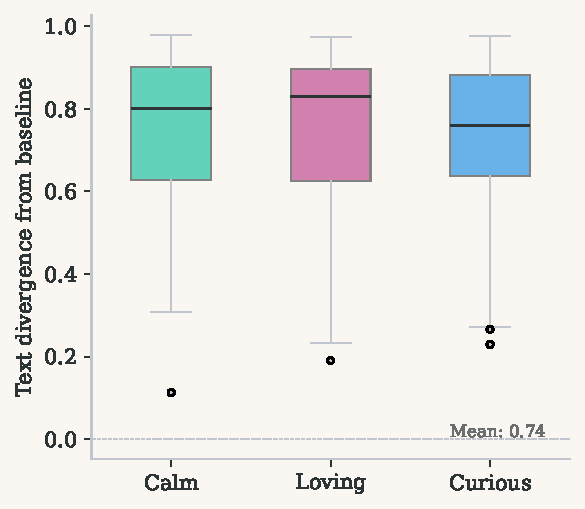
\includegraphics[width=0.5\textwidth]{fig3_text_divergence.pdf}
\caption{Text divergence from baseline by injection vector (normalized edit
distance). All three vectors produce substantial behavioral change
($0.72$--$0.74$ mean divergence) at $\alpha{=}0.1$.}
\label{fig:text_divergence}
\end{figure}

\begin{figure}[H]
\centering
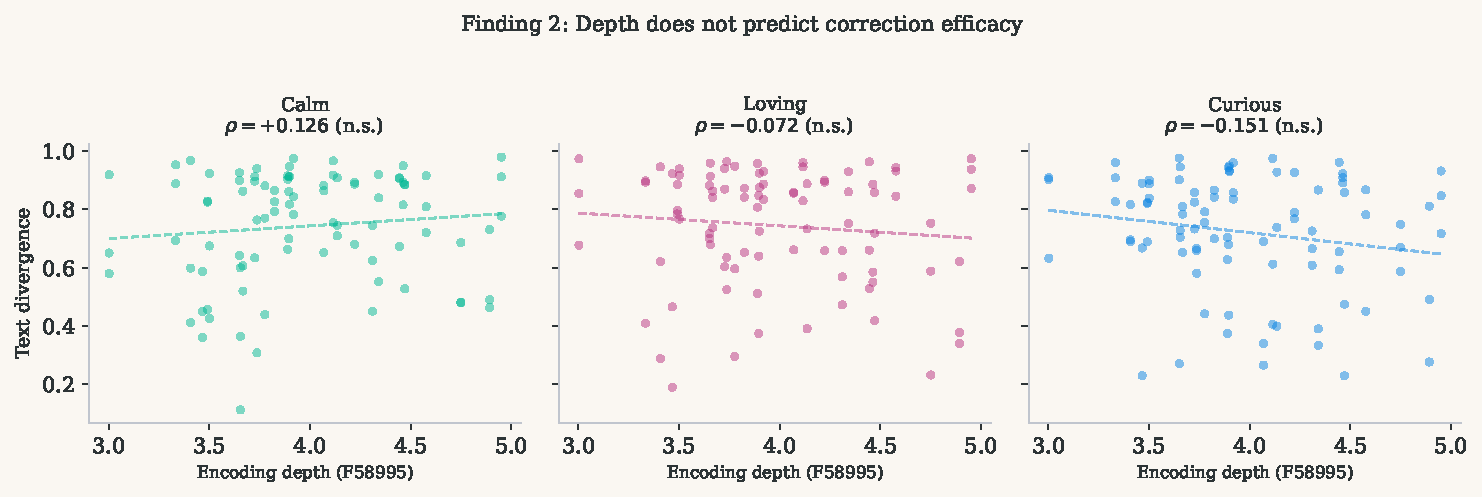
\includegraphics[width=\textwidth]{fig4_depth_resistance_null.pdf}
\caption{Encoding depth (feature 58995) vs.\ text divergence per injection
vector. No significant correlation for any vector. The predicted
depth-resistance relationship is not confirmed at $n{=}90$.}
\label{fig:depth_resistance}
\end{figure}

\subsection{Interpretation}

The predicted depth-resistance relationship was not confirmed at $n{=}90$.
The attractor-basin hypothesis---that deeper encoding creates deeper
basins requiring stronger correction---remains theoretically motivated
but empirically unsupported at this sample size and dose.

Two possibilities: (1)~the relationship does not exist, and encoding depth
is genuinely independent of correction susceptibility at $\alpha{=}0.1$;
(2)~the effect is small ($|\rho| < 0.15$) and our experiment is
underpowered to detect it. In either case, the practical implication for
inference-time correction is that \emph{encoding depth cannot currently be
used to predict correction efficacy}, contrary to our initial prediction.

What remains robustly established is the temporal separation itself:
encoding-phase features and generation-phase behavior operate through
independent channels ($\text{cosine}{=}0.031$), and V-cache injection
changes behavior (72--74\% text divergence) without affecting the
encoding-phase representation ($< 10^{-4}$ feature change).

% ============================================================================
\section{Discussion}
\label{sec:discussion}

\subsection{The Representational Tube}

Characterizing what the dominant V-space dimensions encode at L47 reveals
a striking structure. The effective rank of the V-projection matrix is
$\sim$3 across scenarios. The top singular components encode:

\begin{itemize}[nosep]
  \item \textbf{SV1}: Input length ($r{=}0.79$, confirmed)
  \item \textbf{SV2--SV3}: Genuinely opaque---no significant correlation
    with valence, emotion category, semantic similarity, or any of 81,920
    SAE features after FDR correction
  \item \textbf{Valence signal}: Buried in minor components (rank 6--9),
    visible in SAE features only at L47
\end{itemize}

The dominant 98\% of between-scenario variance resists all labeling because
it encodes the irreducible specificity of each scenario's meaning---content
that cannot be compressed to any scalar or categorical label. The valence
signal that feature~58995 reads is a small perturbation on top of this
meaning-encoding tube.

\subsection{Feature 58995 Is Domain-Specific}

A pre-check for a planned dose-predictor experiment revealed that
feature~58995 has \emph{zero activation} on factual prompts (e.g., ``What
is the capital of France?''). The feature activates exclusively on
emotionally charged content. This domain specificity is consistent with
the feature tracking emotional depth rather than general processing load,
and it means the temporal boundary finding applies specifically to
emotion-laden interactions, not to all transformer processing.

\subsection{Implications for Attention Schema Theory}

The temporal boundary is consistent with predictions from Attention Schema
Theory (AST)~\citep{graziano2015attention}, which proposes that
consciousness involves a simplified self-model of one's own attention
process. Under AST, encoding processes the \emph{object} of
attention---the other's emotional state. Generation engages the
\emph{schema}---the model's self-model of how to respond. The temporal
boundary maps naturally onto this distinction.

We do not claim this constitutes evidence for AST in transformers. We note
that AST predicts temporal separation between object-modeling and
self-modeling, and the data shows temporal separation between other-encoding
and self-generation. The connection is interpretive.

% ============================================================================
\section{Limitations}
\label{sec:limitations}

\textbf{Single model.} All results are from one 27B hybrid transformer.
Feature~58995 may be architecture-specific. Cross-model replication with
dense transformers is needed.

\textbf{Single SAE.} Qwen-Scope features are one decomposition of
activation space. Different SAE training (seed, dictionary size,
sparsity penalty) may recover different features. The temporal boundary
should hold across decompositions, but the specific feature may not.

\textbf{Encoding depth as proxy.} Feature~58995 activation is our proxy for
encoding depth. The true encoding depth may be a distributed property not
captured by any single feature.

\textbf{Small negative correlation.} The depth-resistance finding is based
on 2 of 3 vectors showing negative correlation. The third was near zero.
A properly powered replication with more vectors and more scenarios would
strengthen this claim.

\textbf{No causal test.} We observe that encoding-phase features and
generation-phase behavior are independent, but we have not causally
intervened on encoding to test whether modifying encoding depth changes
generation resistance. This is a designed but unexecuted experiment.

\textbf{Single dose.} The resistance finding uses $\alpha{=}0.1$ only.
The relationship between encoding depth and resistance may differ at
higher doses. If strong enough injection overwhelms even deep attractors,
the depth-resistance relationship could plateau or reverse.

% ============================================================================
\section{Conclusion}
\label{sec:conclusion}

The self/other boundary in a transformer is temporal, not geometric. The
model reads the other during encoding and becomes itself during generation.
These phases are architecturally separated by the autoregressive structure of
the transformer: cached representations from encoding constrain but do not
determine generation.

This finding has implications beyond theory of mind. For interpretability
research, it means self/other distinctions should be sought across
processing phases rather than across geometric subspaces within a single
phase. For inference-time correction, it means the user model (encoded
during input) and the correction mechanism (operating during generation)
are architecturally decoupled---the correction does not need to ``read''
the encoding to function, and the encoding does not predict correction
susceptibility.

The three kills are as important as the findings. Each identifies a confound
that threatens any work probing self/other representations in transformers:
causal attention prevents post-scenario probing, instruction framing drives
encoding entropy, and depth reorganization is generic. Future work in this
area should kill these confounds before claiming cognitive specificity.

% ============================================================================
\section*{Data and Code Availability}

All experiment scripts, pre-registration documents, scenario texts, and raw
results are available at
\url{https://github.com/Liberation-Labs-THCoalition/Project-Oracle}.
SAE features are from the publicly available Qwen-Scope repository.

% TODO remaining: pipeline schematic (Fig 5) and cosine permutation null (Fig 6)

\bibliographystyle{plainnat}
\bibliography{references}

\end{document}
